\section{Case studies}\label{sec:examples}
    The following chapters shows typical use-cases of \ac{scars} Toolbox. First two sections can serve the purpose of teaching with step-by-step instructions how to set-up a simple project. Following parts showcase real life example spacecrafts, of which \ac{aocs} Subsystems can be simulated with blocks from \ac{scars} Parts Library. At the end of the chapter examples of control system tests are presented, proving that \ac{scars} can be used for both prototyping and reviewing processes.

    % \subsection{Initial set-up of ADCS architecture in SCARS}
        % \dots\textit{description}\dots

    \subsection{Simple spacecraft example}\label{sec:simple_spacecraft}
        The nominal usage of \ac{scars} Toolbox is to take a simple objective that designed \ac{aocs} subsystem has to fulfil, choose on board hardware and model the spacecraft accordingly, using only necessary components. To showcase the basic workflow below are presented the steps describing a process to \textbf{check whether chosen set of reaction wheels and gyroscopes can provide} $\pm10$ \textbf{arcminutes accuracy during 10s of geographic coordinates tracking}. The model constructed for this example will be further referred to as Example Model. 

        \subsubsection*{Step 1: Initial Spacecraft Dynamics setup}
            \begin{figure}[H]
                \centering
                \subfloat[Example Model]{{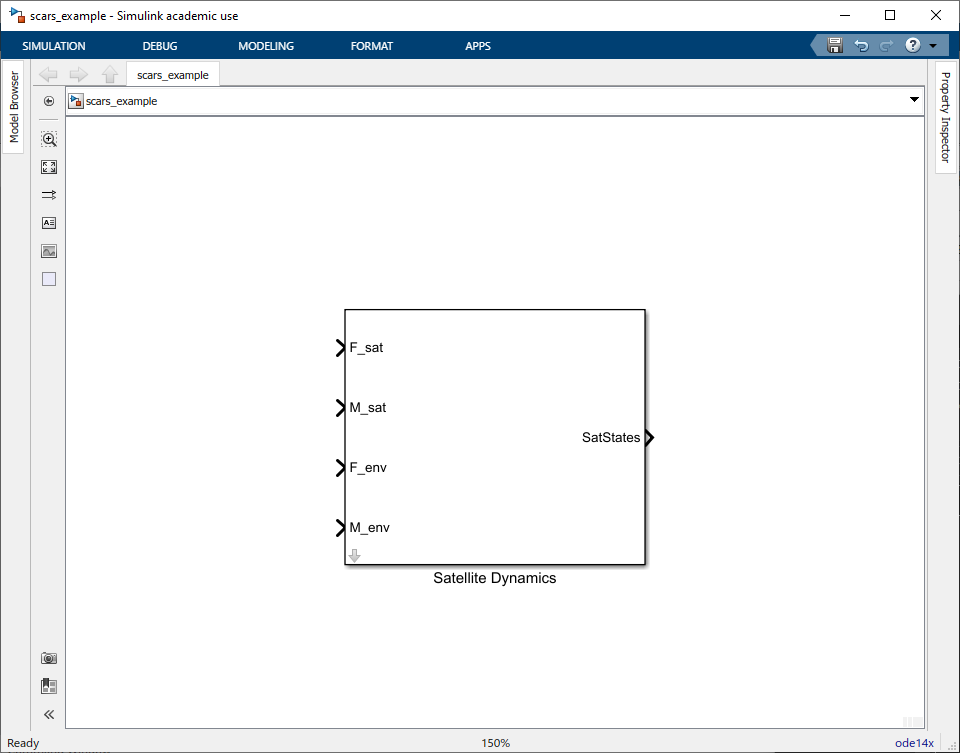
\includegraphics[scale=0.41]{4-examples/01a.png}\label{sub:01a} }}%
                \qquad
                \subfloat[Spacecraft Dynamics Mask]{{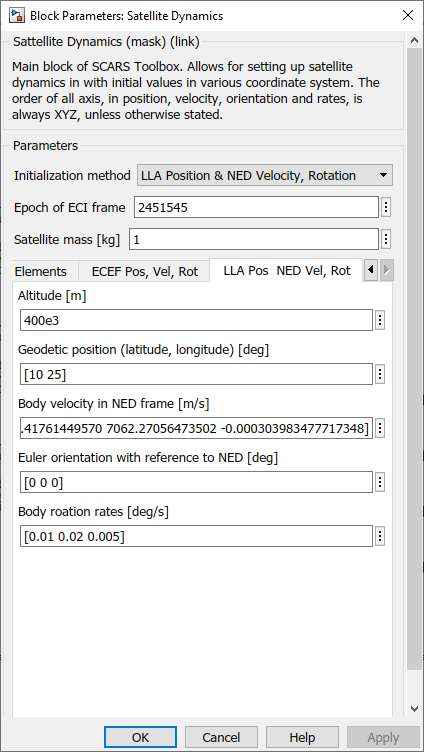
\includegraphics[scale=0.41]{4-examples/01b.png}\label{sub:01b} }}%
                \caption{Step 1}%
                \label{fig:step1}%
            \end{figure}

            To set up the spacecraft as a point in orbit spacecraft dynamics model the user needs to add \textbf{Spacecraft Dynamics} block from \ac{scars} Parts Library, as seen on \autoref{fig:step1} \subref{sub:01a} and to input parameters describing the simulated spacecraft into object's mask. Several initialization methods are available, corresponding to reference frames in which the user can input the data about the starting point. In this case, since the objective is to track geographic coordinates, the method of choice is \textbf{LLA Position \& NED Velocity, Rotation}. The choice of parameters, corresponding to average CubeSat, is presented in \autoref{fig:step1} \subref{sub:01b}. Initial latitude and longitude were chosen arbitrarily, while still in the neighborhood of the point to be tracked.
            
            Afterwards the user can set up Simulink model solver parameters to \textbf{Fixed-step} with \textbf{ode14x} solver choice, while leaving the rest with default settings. While not being necessary, it allows larger step-size when using \textbf{Derivative} blocks.
            % the screenshot filled \textbf{Spacecraft Dynamics} Simulink mask.

        \subsubsection*{Step 2: Environment setup}
            \begin{figure}[H]
                \centering
                \subfloat[Example Model]{{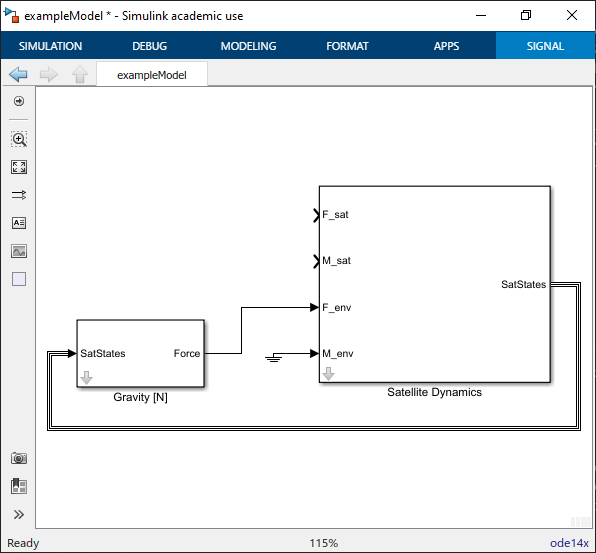
\includegraphics[scale=0.41]{4-examples/02a.png}\label{sub:02a} }}%
                \qquad
                \subfloat[Gravity Mask]{{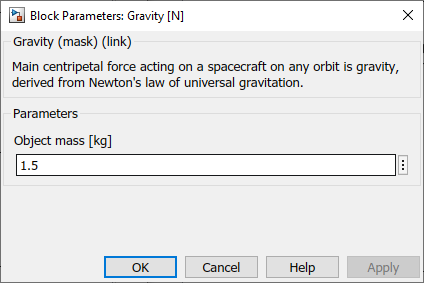
\includegraphics[scale=0.41]{4-examples/02b.png}\label{sub:02b} }}%
                \caption{Step 2}%
                \label{fig:step2}%
            \end{figure}

            This spacecraft does not use magnetorquers nor does not have any major drag-inducing components, therefore the relevant block representing environment's influence on the satellite is the \textbf{Gravity [N]} block. The only parameter to input is spacecraft's mass, as seen on \autoref{fig:step2} \subref{sub:02a}.

        \subsubsection*{Step 3: Actuators choice and setup}
            \begin{figure}[H]
                \centering
                \subfloat[Example Model]{{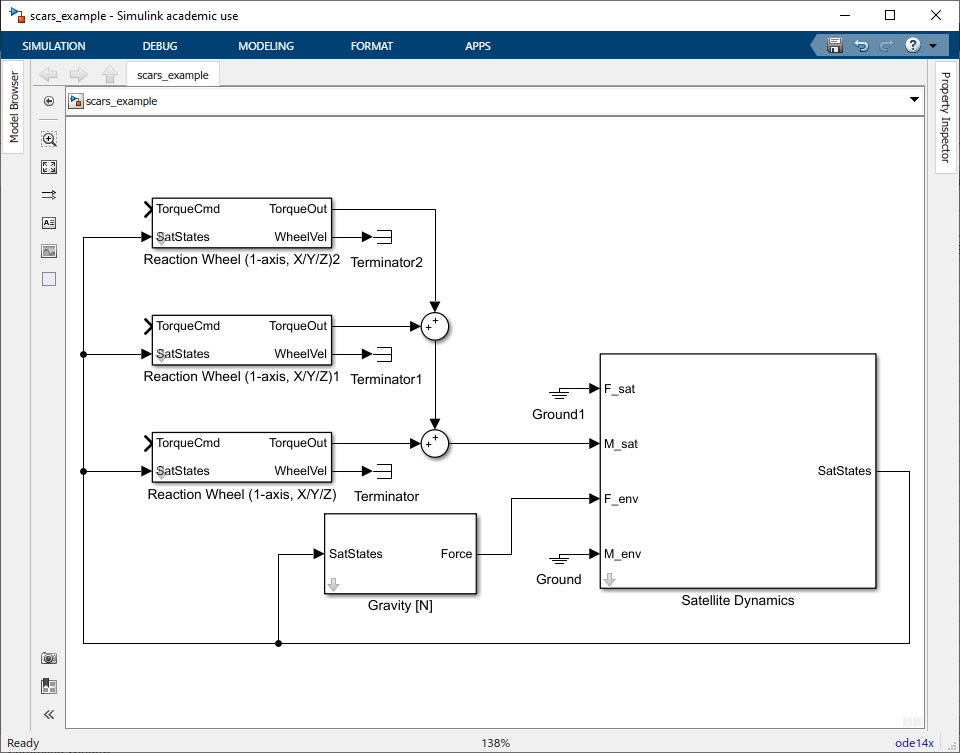
\includegraphics[scale=0.41]{4-examples/03a.png}\label{sub:03a} }}%
                \qquad
                \subfloat[Reaction Wheel Mask]{{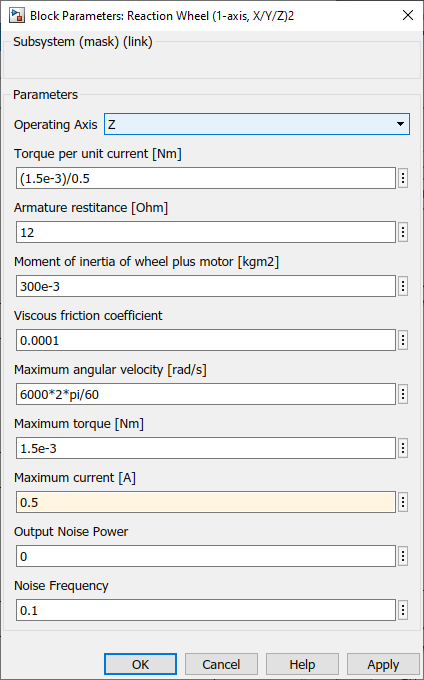
\includegraphics[scale=0.41]{4-examples/03b.png}\label{sub:03b} }}%
                \caption{Step 3}%
                \label{fig:step3}%s
            \end{figure}

            The next step is to implement the choice of actuators into the spacecraft model. In this example the user might want to test the NanoTorque GSW-600 reaction wheels, in nominal configuration of one wheel for each spacecraft body axis, from GomSpace manufacturer. The list of relevant parameters, compiled from the actuator's datasheet, can be seen on \autoref{fig:step3} \subref{sub:03b}. They were put into as parameters of \textbf{Reaction Wheel (1 axis X/Y/Z)} block from \ac{scars} Parts Library and added to Example Model. The required inputs are the control signal and \textbf{SatStates} bus signal (described in \autoref{sec:space_mechanics}), while the outputs are torque and wheel angular rate.

            % here be table with citation to the datasheet
        
        \subsubsection*{Step 4: Setup of control algorithm}
            \begin{figure}[H]
                \centering
                \subfloat[Example Model]{{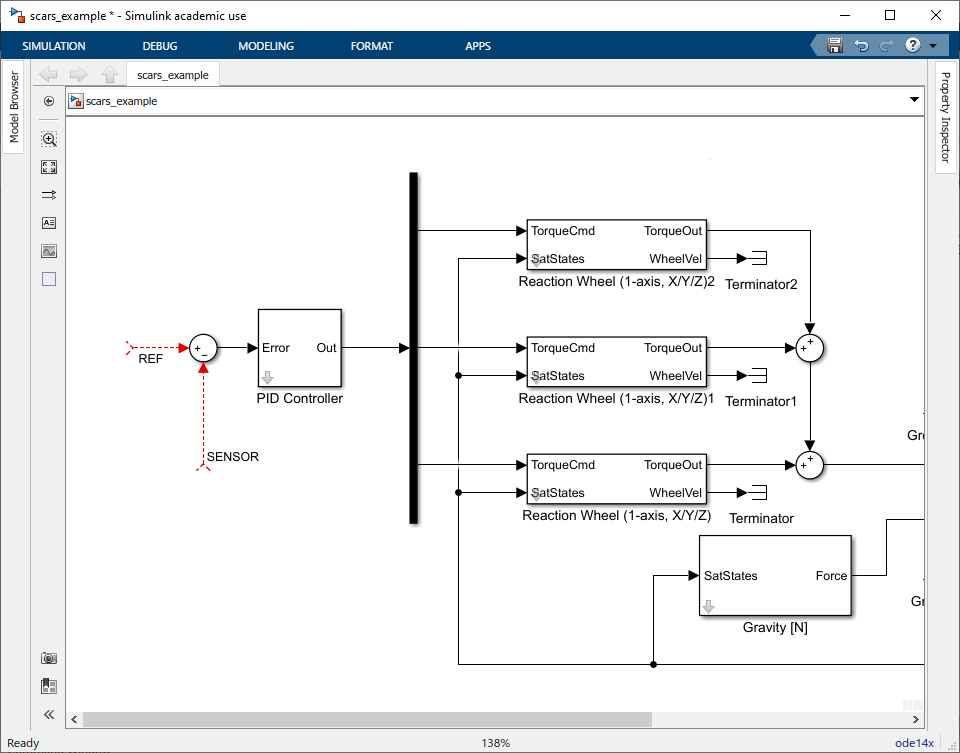
\includegraphics[scale=0.4]{4-examples/04a.png}\label{sub:04a} }}%
                \qquad
                \subfloat[PID Mask]{{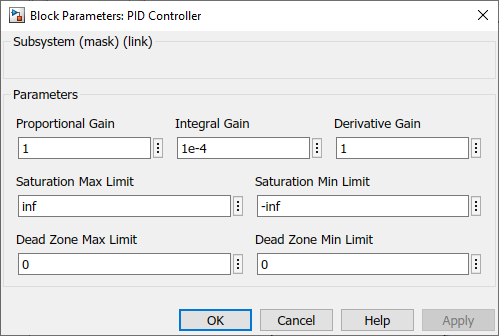
\includegraphics[scale=0.40]{4-examples/04b.png}\label{sub:04b} }}%
                \caption{Step 4}%
                \label{fig:step4}%
            \end{figure}
            A \ac{pid} controller was chosen as a control mechanism for reaction wheels. \autoref{fig:step4} \subref{sub:04b} represents the initial set up of the parameters of this conroller block. Saturation of \textbf{PID Controller} output signal was set up in accordance to hardware's maximum voltage.

        \subsubsection*{Step 5: Coordinate transformation and reference signal}
            \begin{figure}[H]
                \centering
                \subfloat[Example Model]{{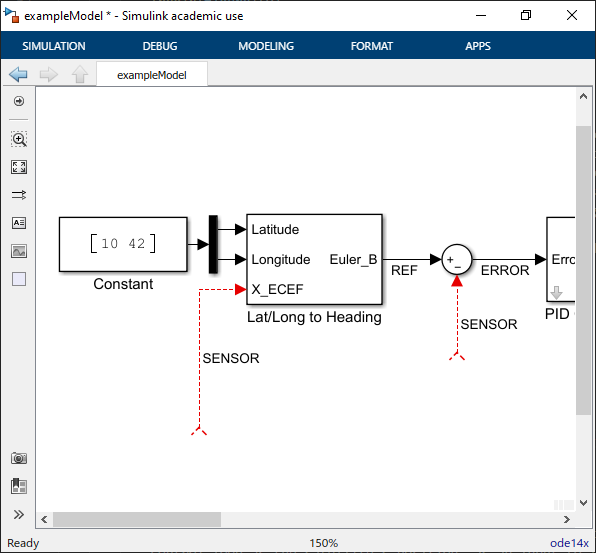
\includegraphics[scale=0.41]{4-examples/05a.png}\label{sub:05a} }}
                \caption{Step 5}%
                \label{fig:step5}%
            \end{figure}
            \ac{scars} Toolbox also provides a way to speed up the process of building mathematical transformations, allowing the user to conduct initial tests first and to design the software implementation afterwards. This approach leads to significant savings in amount of work to be performed by the control system engineer, as failing solutions can be rejected without spending time on setting up algorithms from scratch. In this case, \textbf{Lat/Long to Heading} block was used, without the need for any further setup. As first two inputs are the desired geographical coordinates and the last one is the position vector of the satellite, in \ac{ecef} reference system.

        \subsubsection*{Step 6: Sensors choice and setup}
            \begin{figure}[H]
                \centering
                \subfloat[Example Model]{{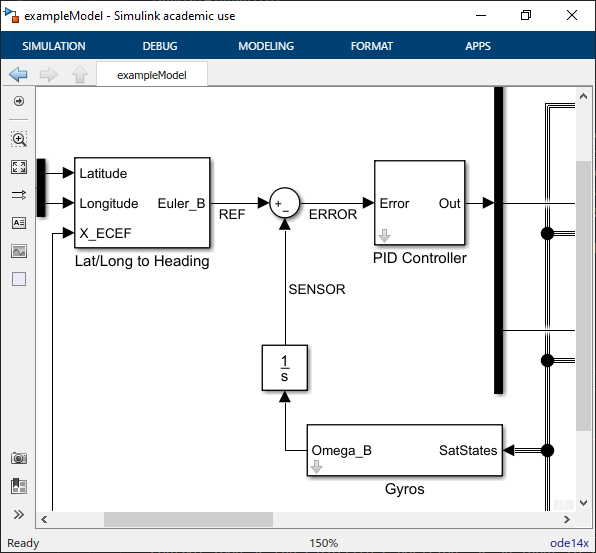
\includegraphics[scale=0.41]{4-examples/06a.png}\label{sub:06a} }}%
                \qquad
                \subfloat[Gyros Mask]{{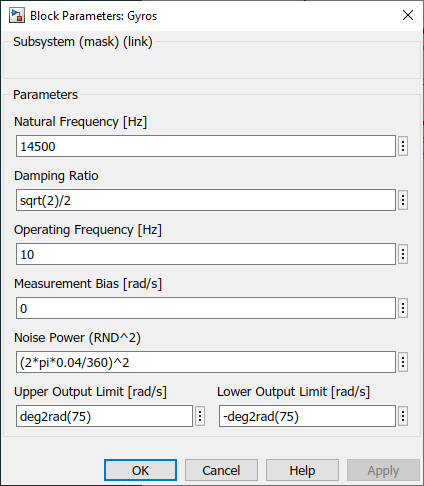
\includegraphics[scale=0.41]{4-examples/06b.png}\label{sub:06b} }}%
                \caption{Step 6}%
                \label{fig:step6}%
            \end{figure}
            Figure \autoref{fig:step5} shows that the only signals necessary to close the control loop as the satellite's position, as an input to \textbf{Lat/Long to Heading}, and Euler angles in body reference frame. The former is irrelevant to the posed objective of this Example Model, therefore was set up to be measured by the \textbf{Ideal Position Sensor (ECEF)} block, and the latter had to be the analysed gyroscope. \textbf{Gyros} block was added to the simulation and set up with the parameters of the gyroscope, chosen by the fictitious user to be ADXRS614 MEMS Gyroscope, as proposed by Li et al\cite{li2013design}.
            
            The extract from the datasheet and it's representation as \ac{scars}' block parameters can be found on \autoref{fig:step6} \subref{sub:06a} and \autoref{fig:step6} \subref{sub:06b} respectively.

        \subsubsection*{Step 7: Simulation and verification}
            Finally, the simulation has to be run by the user and the results can be verified. The model is simulated to track reference geographic position of $10$ degrees of latitude and $40$ degrees of longitude. The satellite progresses over geographical coordinates as presented on \autoref{fig:angleandposition} \subref{sub:example_geo}, which results in calculated reference angle visible on \autoref{fig:angleandposition} \subref{sub:example_ref}.

            \begin{figure}[H]
                \centering
                \subfloat[Geographical position of the satellite]{{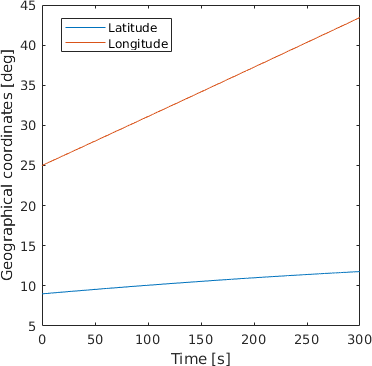
\includegraphics[scale=0.44]{4-examples/example_geo.png}\label{sub:example_geo} }}%
                \qquad
                \subfloat[Satellite reference body angle]{{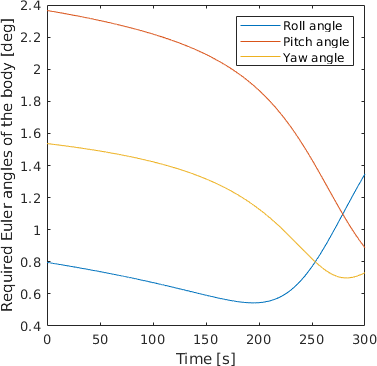
\includegraphics[scale=0.44]{4-examples/example_ref.png}\label{sub:example_ref} }}%
                \caption{Data used for and produced by tracking subsystem}%
                \label{fig:angleandposition}%
            \end{figure}
                         
            \begin{figure}[H]
                \centering
                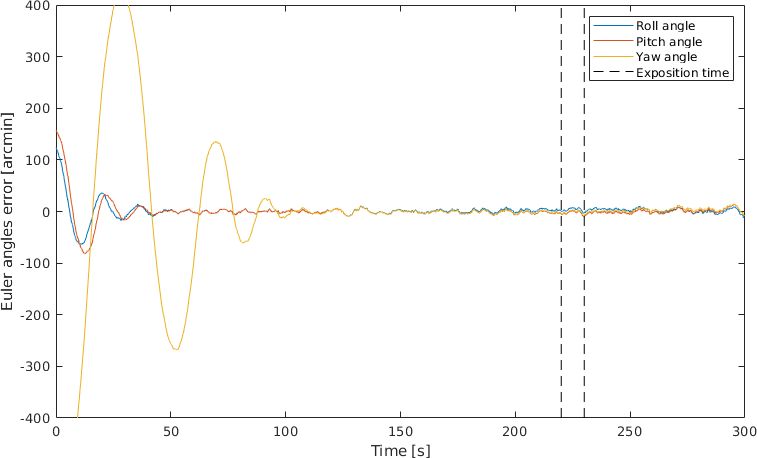
\includegraphics[width=1\textwidth, height=160px]{4-examples/example_error.png}
                \caption{Plot of Euler angle error against reference angles, derived from geographical coordinates and satellite position}
                \label{fig:example_error}
            \end{figure}

            \autoref{fig:example_error} shows the results from Example Model simulation. It is assumed that the satellite has attained attitude close to required during previous orbit, to mitigate the possibility of high body rates achieved during reference tracking rise time. During the first minute the satellite reaches accuracy under $1$ degree and the error decreases.
                         
            \begin{figure}[H]
                \centering
                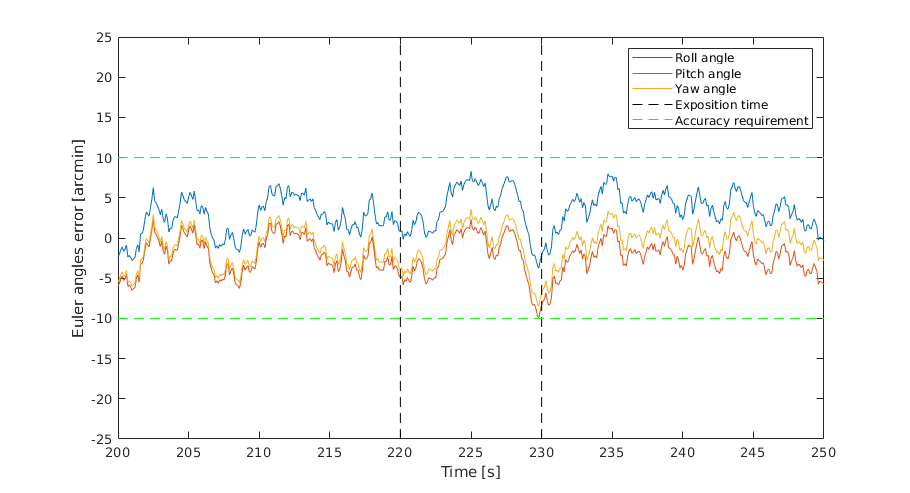
\includegraphics[width=1\textwidth, height=160px]{4-examples/example_zoom.png}
                \caption{Plot of Euler angle error against reference angles, derived from geographical coordinates and satellite position, in focus on time between 200 and 250 seconds}
                \label{fig:example_zoom}
            \end{figure}

            The resulting plot is magnified to focus on simulation time between $200$ and $250$ seconds. It can be observed that for $10$ seconds of marked timing the accuracy of the control system maintains the angle within $\pm 10$ arcminutes. While this can be considered satisfactory and concludes this example, it is possible to improve the response of the system using methods presented in \autoref{sec:test_examples}.
 
            % \dots\textit{finish description}\dots





    \subsection{PW-Sat2}\label{sec:pwsat2}
        % Magnetorquers
        As written on its website, "PW-Sat2 is a student satellite project started in 2013 at Warsaw University of Technology by the Students Space Association members. Its main technical goal is to test new deorbitation technology in form of a large deorbitation sail whereas the project purpose is to educate a group of new space engineers. In February 2018 PW-Sat2 became fully integrated and was being prepared to the launch into orbit planned for the second half of 2018."\cite{pwsat2website}
        % https://pw-sat.pl/wp-content/uploads/2014/07/PW-Sat2-C-01.00-ADCS-CDR.pdf
                         
        \begin{figure}[H]
            \centering
            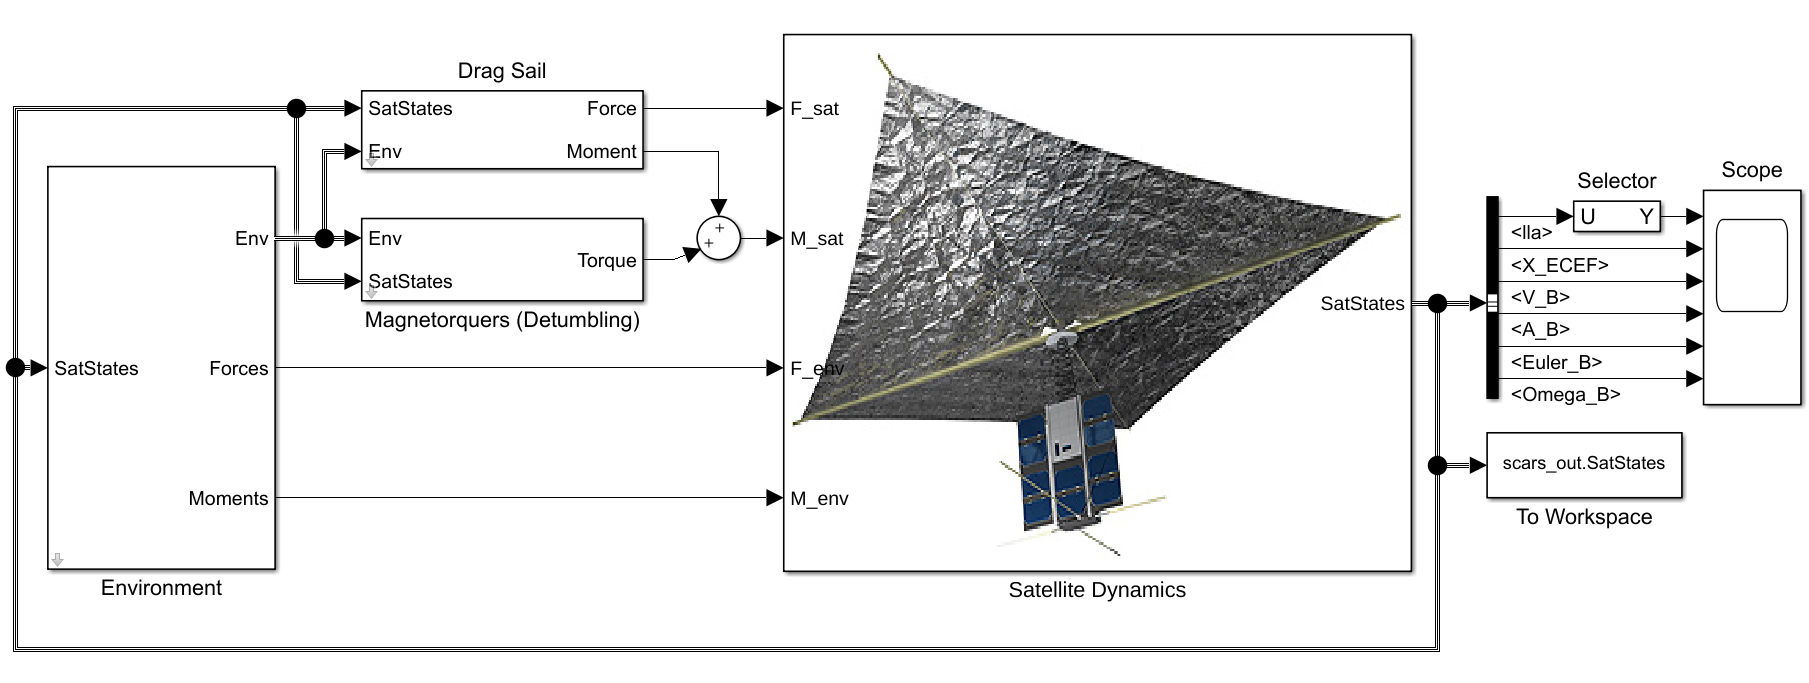
\includegraphics[width=1\textwidth]{4-examples/pwsat2model.png}
            \caption{PW-Sat2 model created with components from SCARS Parts Library}
            \label{fig:pwsat2model}
        \end{figure}

        As it can be seen on \autoref{fig:pwsat2model}, PW-Sat2 Simulink model is build exclusively from parts available \ac{scars} toolbox, save for connecting blocks. It contains \textbf{Satellite Dynamics} block as the core of the simulation and it is set up using Keplerian elements taken from PW-Sat2 first \ac{tle} frame. Apart from that, full SCARS \textbf{Environment} model is included and connected to two actuators: \textbf{Drag Sail} and \textbf{Magnetorquers (Detumbling)}. \autoref{fig:pwsat2actuators} shows the setup of actuators' parameters - sources of these values are described in following sections. 

        
        \begin{figure}[H]
            \centering
            \subfloat[Drag Sail block mask]{{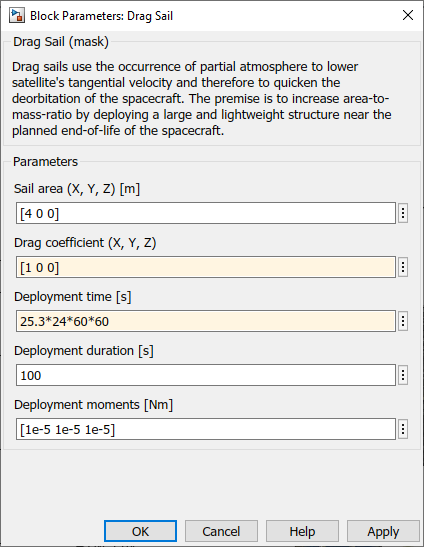
\includegraphics[scale=0.44]{4-examples/pwsat2dragsail.png}\label{sub:pwsat2dragsail} }}%
            \qquad
            \subfloat[Magnetorquers (Detumbling) block mask]{{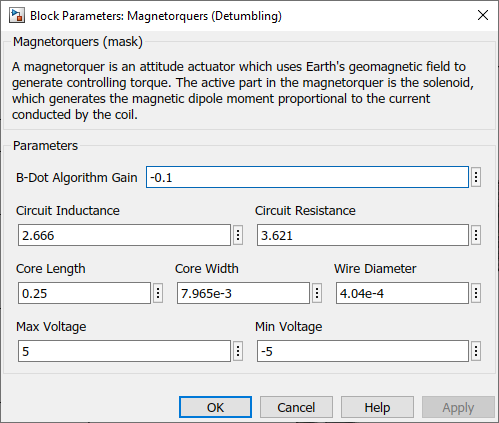
\includegraphics[scale=0.44]{4-examples/pwsat2magne.png}\label{sub:pwsat2magne} }}%
            \caption{Parameters of SCARS PW-Sat2 model}%
            \label{fig:pwsat2actuators}%
        \end{figure}

        \subsubsection{Detumbling}
            One of two modes of control that PW-Sat2 operates in (with the other one being Sun Pointing Mode) is Detumbling Control Mode. Detumbling maneuver is performed after deployment of the spacecraft from a carrier rocket. As the satellites are separated from the deployment mechanism, they are burdened by non-zero initial angular rates. To counteract that and stabilize a satellite PW-Sat2 is equipped with a set of two perpendicular magnetorquer rods and one air core, in total one coil acting along each of satellite's body axis. The crucial parameters used by \ac{scars} model of PW-Sat2 are listed in Table \ref{table:pwsat2magne}.\cite{pwsat2adcs} Exact values are taken directly from the datasheet of \ac{imqt} \cite{imqt-datasheet}, as it was the magnetorquer used by PW-Sat2. Since \ac{scars} contains only model for magnetorquer rods, the air core magnetorquer was assumed to be another torque rod. Also, since not every parameter of magnetorquer could be found in the datasheet, the missing fields were filled with data from similar ones.

            \begin{table}[H]
                \centering    
                \small
                \begin{tabular}{l l}
                    \textbf{Parameter} & \textbf{Value} \\ \hline
                    Nominal magnetic dipole & $0.2 Am^2$ \\
                    Maximum actuation envelope error & $3\mu T$ \\
                    Power consumption during actuation & $1.2W$ \\
                    Maximum operating voltage & $5V$ \\
                    Mass & 196g \\ \hline
                \end{tabular}
                \caption{Parameters gather from magnetorquer board installed on PW-Sat2}\label{table:pwsat2magne}
            \end{table}

            As it can be seen on \autoref{fig:detumble}, detumbling was mostly successful, with small angular rates remaining on each axis. Such result is possible, since change in magnetic field on magnetorquers is proportional to the angular rate of the spacecraft, so when spacecraft is rotating slowly the torque generated by the actuator is also minor. Given enough time the satellite should approach near-zero rotation rate, but resulting value should be enough for good connection with the ground station to transfer into more active control mode. 

            \begin{figure}[H]
                \centering
                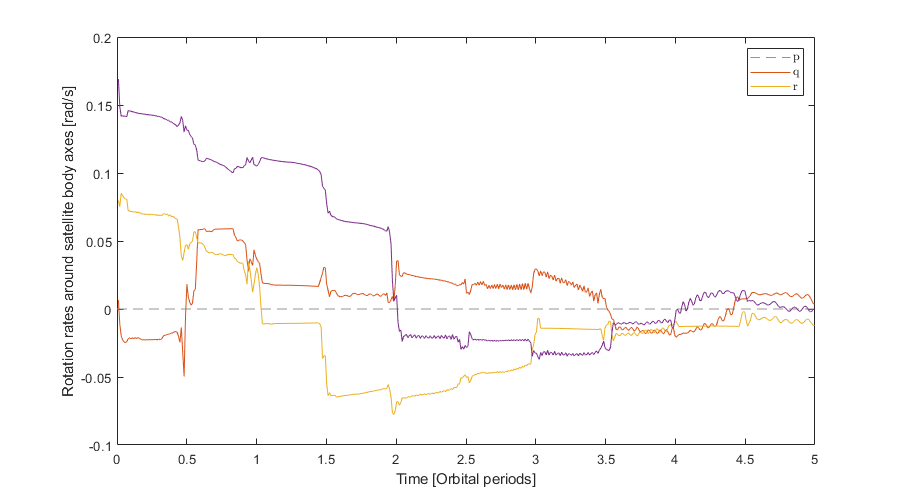
\includegraphics[width=1\textwidth, height=160px]{4-examples/pwsat2-detumble.png}
                \caption{Results from \ac{scars} simulation, with magnetorquers set up for detumbling}
                \label{fig:detumble}
            \end{figure}

        \subsubsection{Deorbitation with drag sail}
            One of the main objectives of PW-Sat2 mission was to deploy and test the effectiveness of its drag sail in deorbitation maneuver. The sail was  $2$x$2m$ square made from aluminized polyester boPET film\cite{pwsat2dt}.
            
            In this example, \ac{scars} toolbox was tested against data points derived from NORAD measurements. The simulation was run with the drag sail set up to be deployed around 25th day of the mission.
                         
            \begin{figure}[H]
                \centering
                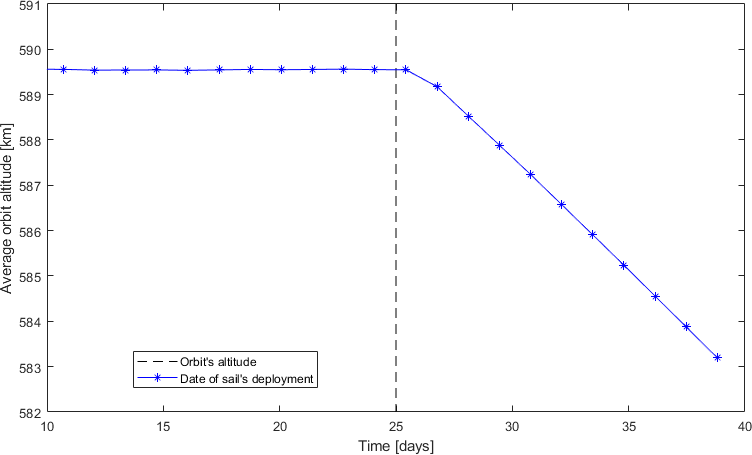
\includegraphics[width=1\textwidth, height=160px]{4-examples/scars-deorbit.png}
                \caption{Results from \ac{scars} simulation, with drag sail included}
                \label{fig:scars-deorbit}
            \end{figure}

            Since sail's deployment the forementioned decrease of satellite's attitude is presented in \autoref{fig:pw-sat-deorbit}, showing the proof of deceleration caused by the sail. When comparing results from \ac{scars} simulation with data collected from PW-Sat2 \ac{tle}s, visible on \autoref{fig:pw-sat-deorbit} it is apparent that attitude changes are much more brisk in \ac{scars} model than in real life. Such results were to be expected, as in PW-Sat2, shortly after deployment the sail has torn, therefore the effective drag was much lower than simulated value\cite{space24_pwsat}. Also, since TLE data is a mixture of propagation and observation, the rate of descent is not accurate for the first few days after sail's deployment. In addition to that, simulated results may seem much smoother, as they the data points are averaged over duration of $10$ orbits, when TLE data points are located arbitrarily.
            
            \begin{figure}[H]
                \centering
                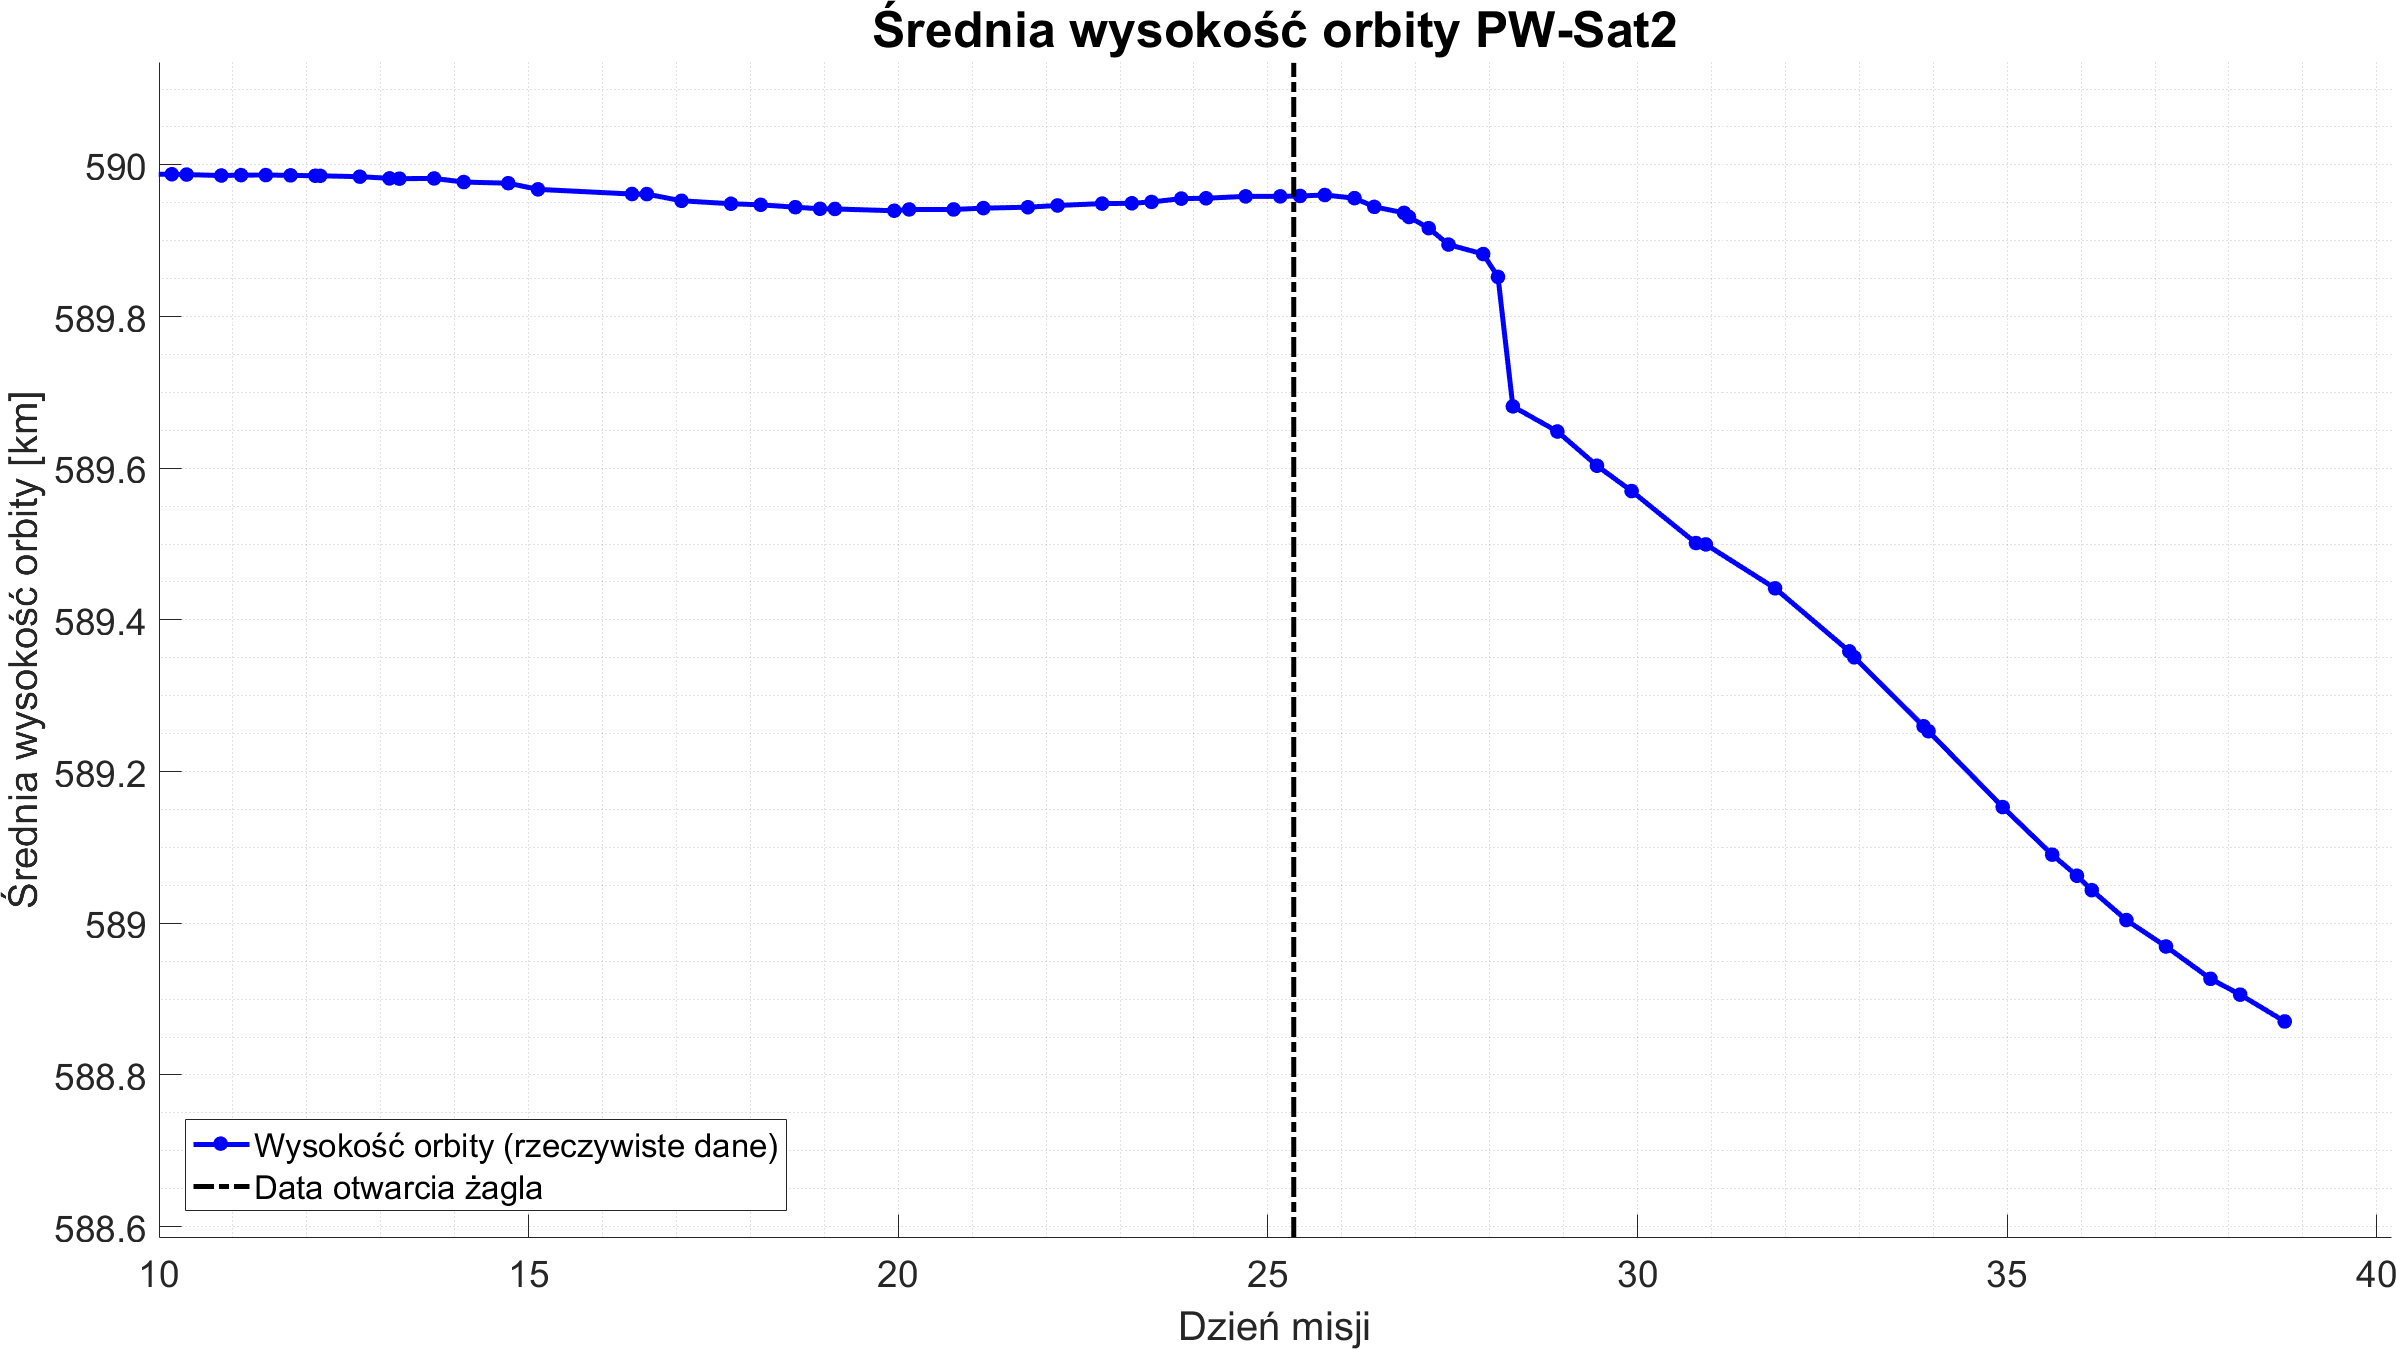
\includegraphics[width=1\textwidth]{4-examples/pw-sat-deorbit.png}
                \caption{Average altitude of PW-Sat2 satellite as taken from \ac{norad} measurements. On X axis there is mission time in days, on Y axis there is an average altitude in km\cite{pw_sat2_deorbit}}
                \label{fig:pw-sat-deorbit}
            \end{figure}

            Simulation of PW-Sat2 deorbitation showcases the SCARS Toolbox' ability of performing long-term simulation.
            
            % \begin{figure}[H]
            %     \centering
            %     \includegraphics[width=1\textwidth, height=160px]{example-image-b}
            %     \caption{Results from \ac{scars} simulation, with magnetorquer-driven attitude correction}
            %     \label{fig:scars-deorbit3}
            % \end{figure}


        % \subsubsection{PROBA-1}
        % https://directory.eoportal.org/web/eoportal/satellite-missions/p/proba-1#spacecraft







    \subsection{Sentinel-2}\label{sec:sentinel}
    
        Sentinel-2 is an European polar satellite mission carried out by \ac{esa} as a part of Copernicus Programme. It consists of constellation of twin polar orbit satellites, Sentinel-2A and Sentinel-2B and its aim is to deliver Earth observation data to broad public, providing wide range of services such as natural emergency management, agricultural monitoring or water classification\cite{sentinel2user}.

        As per document describing Sentinel-2 \ac{adcs} subsystem, the satellites operate on a sun-synchronous orbit, with $786km$ mean altitude and $10:30$ local time of descending node. They maintain Earth-oriented attitude in all operational modes. The required pointing performance is moderate, but the main design driver is the need for precise geo-location of the images\cite{wiedermann2014sentinel}. The actuators and sensors on board of Sentinel-2 are described in Table \ref{table:sentinel-adcs}.

        % Gyro: https://spaceequipment.airbusdefenceandspace.com/avionics/fiber-optic-gyroscopes/astrix-200/
        % Thrusters: https://www.yumpu.com/en/document/read/10860453/1-n-monopropellant-thruster-astrium-st-eads
        % Magnetometer: http://www.zarmtec.uni-bremen.de/products/magnetometer/
            
        \begin{table}    
            \small
            \begin{tabularx}{\textwidth}{ c l X l l }
                \textbf{No.} & \textbf{Uni}t & \textbf{Type} & \textbf{Supplier} & \textbf{Name} \\ \hline
                3 & MAG & 3-axis fluxgate magnetometer & ZARM Technik & FGM-A-75 \\
                2 & GPRS & 2 band GPS receiver & RUAG & - \\
                3 & STR  & Active pixel sensor star tracker & Jena Optronik & Astro APS \\
                4 & IMU & High performance fibre optical gyro & Astrium & ASTRIX 200 \\
                3 & MTQ & $140 Am^2$ magnetic torquer & ZARM Technik & MT140-2\\
                4 & RW & $18 Nms$ reaction wheel & Honeywell & HR12 \\
                8 & THR & $1N$ monopropellant thruster & EADS ST &CHTIN-6 \\ \hline
            \end{tabularx}
            \caption{Actuators and sensors on board of Sentinel-2 spacecraft\cite{wiedermann2014sentinel}}\label{table:sentinel-adcs}
        \end{table}

        Using that data, the model was created using \ac{scars} Parts Library. It was created purely for demonstration purposes, to prove that this toolbox can be used not only for small satellite missions, but also for purposes of scientific and commercial satellites. As one can see in \autoref{fig:sentinel}, the connections between \textbf{Satellite Dynamic} model, \textbf{Environment} block, \textbf{Sensors} and \textbf{Actuators} subsystems are solved with signal buses described in \autoref{sec:buses}.
        
        \begin{sidewaysfigure}
            \centering
            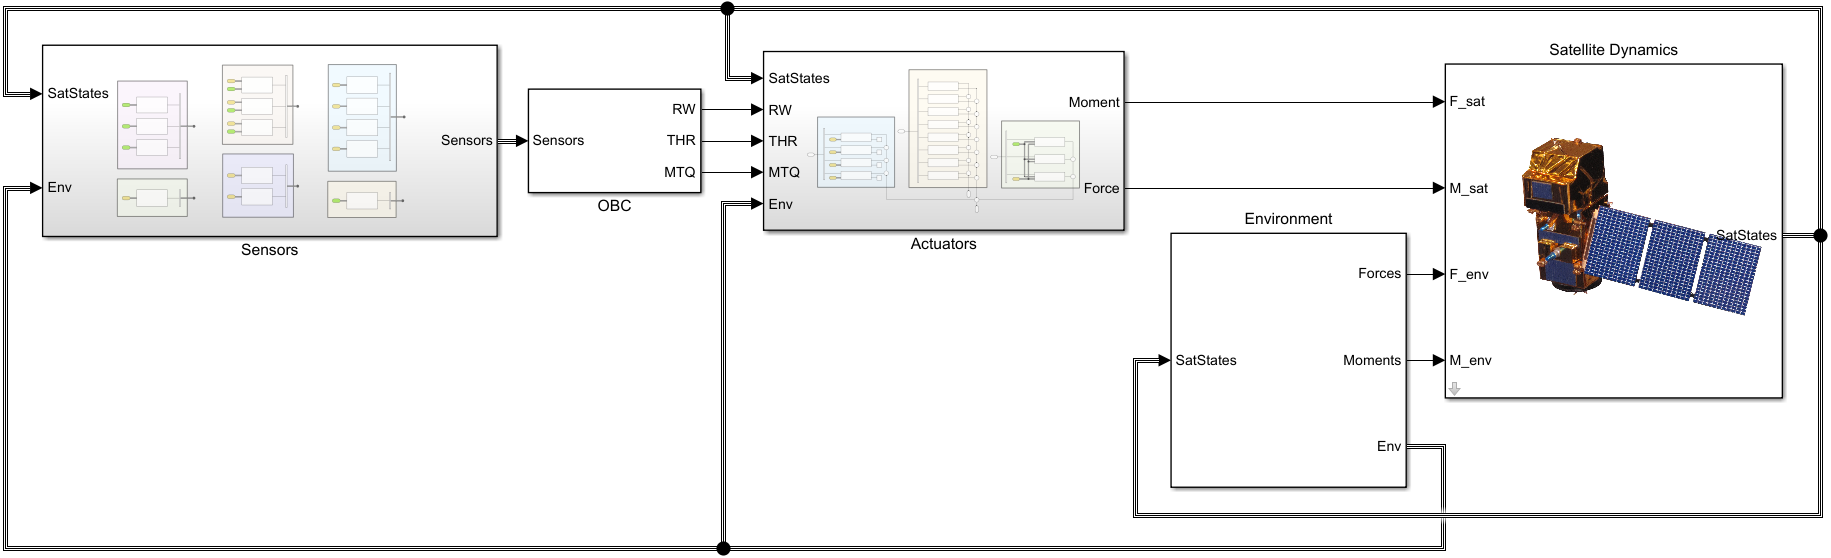
\includegraphics[width=1\textwidth]{4-examples/sentinel.png}
            \caption{Sentinel-2 satellite ADCS model top-level view}
            \label{fig:sentinel}
        \end{sidewaysfigure}

        The subsystems can be explored, showing the setup of SCARS block responsible for sensors in \autoref{fig:sentinel_sensors} and actuators in \autoref{fig:sentinel_actuators}. Since the model serves for example only, it is not fully functional, as on board computer and state machine responsible for sensor fusion and for fault detection and isolation is not recreated in the model - reproducing algorithms behind this could be a topic for another thesis.  Also, one can notice that Sentinel-2 model includes a sun sensor model. In current version of SCARS it could be only implemented by using \textbf{Ideal Sensor} block.
        
        \clearpage
        \begin{sidewaysfigure}
            \centering
            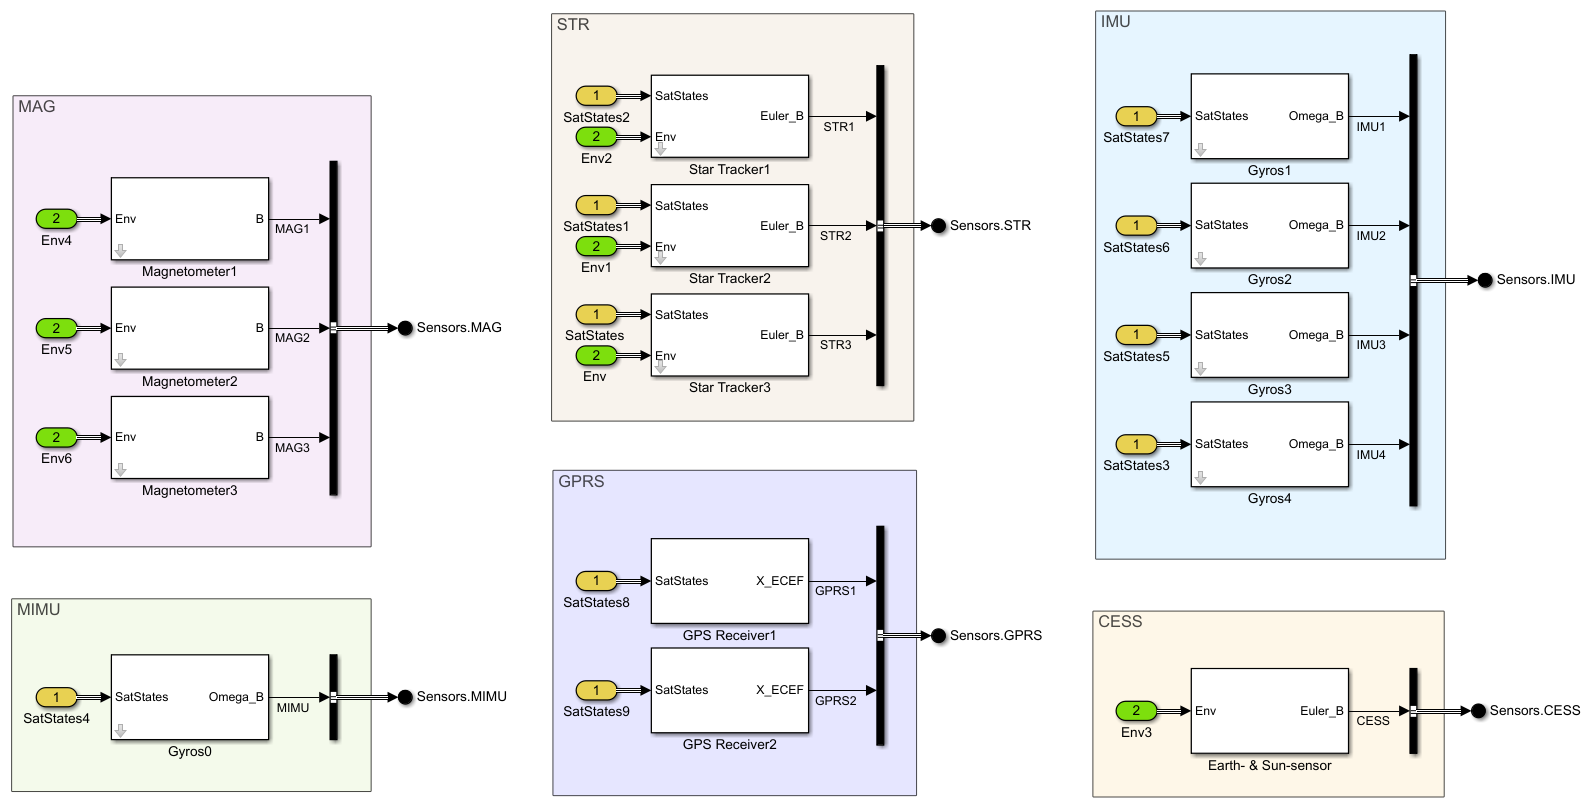
\includegraphics[width=\textwidth]{4-examples/sentinel_sensors.png}
            \caption{Sentinel-2 satellite ADCS model, Sensors subsystem}
            \label{fig:sentinel_sensors}
        \end{sidewaysfigure}
        \clearpage
        \begin{sidewaysfigure}
            \centering
            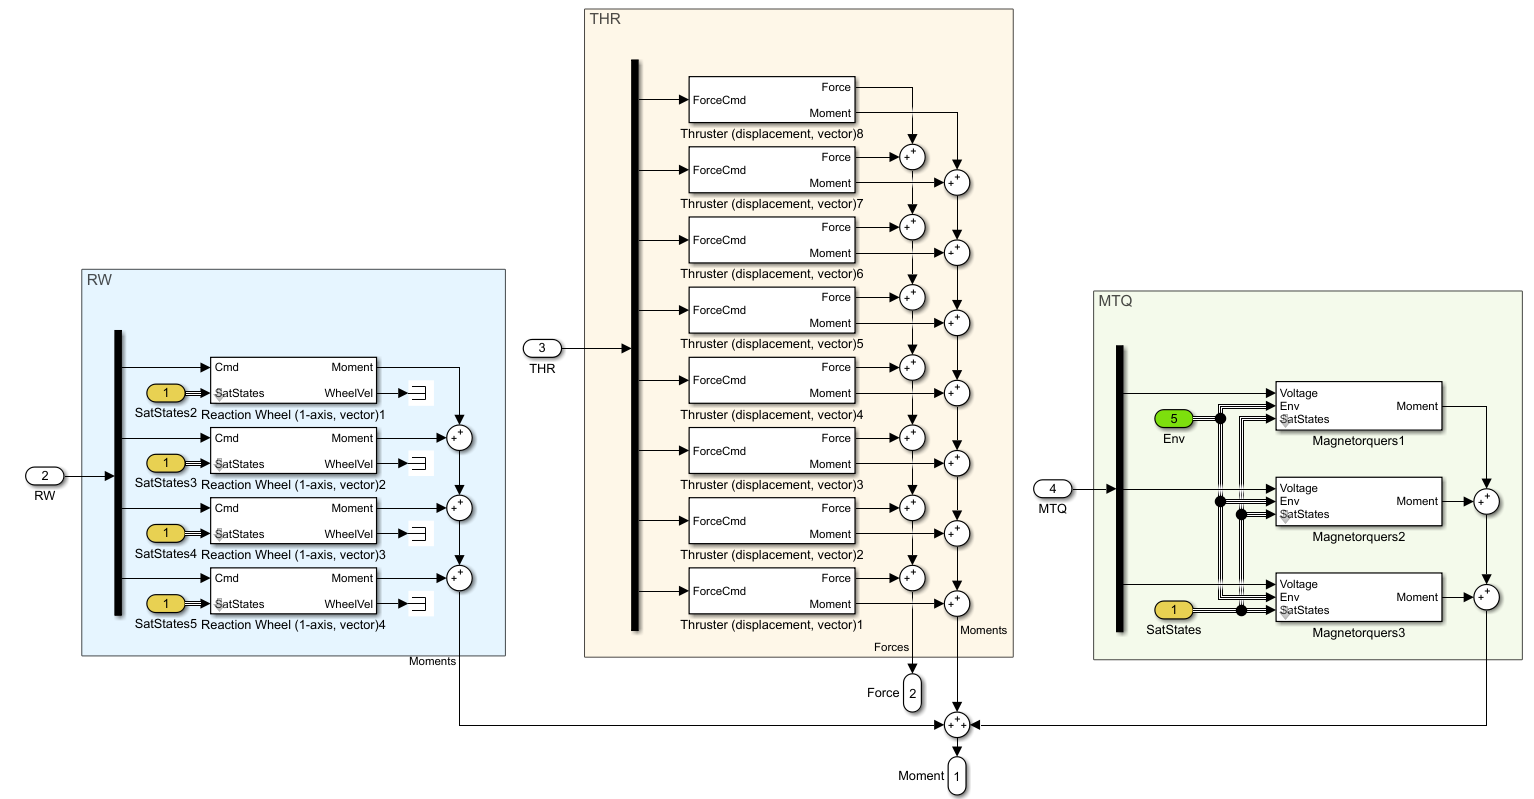
\includegraphics[width=\textwidth]{4-examples/sentinel_actuators.png}
            \caption{Sentinel-2 satellite ADCS model, Actuators subsystem}
            \label{fig:sentinel_actuators}
        \end{sidewaysfigure}
        \clearpage








\subsection{Other application of SCARS Toolbox}\label{sec:test_examples}
    % \dots\textit{introduction}\dots
    % todo: introduction
    While previous sections provide examples for which whole spacecrafts models had to be constructed, the following examples show how SCARS Toolbox can be used to conduct further tests on already prepared models. 

    \subsubsection{Controller design using linearized model}\label{sec:control_design}
        In \autoref{sec:simple_spacecraft}, the gains in PID controller for reaction wheels were set up basing on empirical analysis, rather than on any tuning method. Alternative to that would be to use the linearization method described in \autoref{app:linearization} and Control System Designer, which is available as a part of MATLAB Control System Toolbox. To showcase this possibility Example Model from previous chapter was linearized according to appendix, with resulting state-space representation:
        \small
        \begin{equation}
            A =
            \begin{bmatrix}
                2.5e \text{-}6 &            0 &            0 &      7.5e \text{-}7  &           0  &           0            & 0            & 0           &  0 \\
                      0 &     -2.5e \text{-}6 &            0 &            0  &     7.5e \text{-}7  &           0            & 0            & 0           &  0 \\
                      0 &            0 &     -2.5e \text{-}6 &            0  &           0  &     7.5e \text{-}7            & 0            & 0           &  0 \\
                2.5e \text{-}6 &            0 &            0 &     -7.5e \text{-}7  &           0  &           0            & 0            & 0           &  0 \\
                      0 &      2.5e \text{-}6 &            0 &            0  &    -7.5e \text{-}7  &           0            & 0            & 0           &  0 \\
                      0 &            0 &      2.5e \text{-}6 &            0  &           0  &    -7.5e \text{-}7            & 0            & 0           &  0 \\
                      0 &            0 &            0 &            1  &           0  &           0            & 0            & 0           &  0 \\
                      0 &            0 &            0 &            0  &           1  &           0            & 0            & 0           &  0 \\
                      0 &            0 &            0 &            0  &           0  &           1            & 0            & 0           &  0 
            \end{bmatrix}
        \end{equation}
        \normalsize
        
        \small
        \begin{equation}
            B = 
            \begin{bmatrix}
                \text{-}0.00025  &           0 &            0 \\
                       0  &     \text{-}0.00025 &            0 \\
                       0  &           0 &      \text{-}0.00025 \\
                 0.00025  &           0 &            0 \\
                       0  &     0.00025 &            0 \\
                       0  &           0 &      0.00025 \\
                       0  &           0 &            0 \\
                       0  &           0 &            0 \\
                       0  &           0 &            0
            \end{bmatrix}
        \end{equation}
        \normalsize
    
        Where rows from 1 to 3 represent for reaction wheels angular rates, from 4 to 6 for satellite angular rates and from 7 to 9 for body angles. Said system can be put into controller-plant feedback loop on figure \autoref{fig:feedback} in form $G = Ax + Bu$. The minimal realization of a transfer function of this system can be approximated to $G(s) = \frac{2.5\cdot10^{-4}}{s(s+3.25\cdot10^{-6})}$. The response is very close to an ideal double integrator, with some damping coming from losses inside the reaction wheels, coming from simulated losses on the circuits and mechanical components. 
        
        In the loop presented on \autoref{fig:feedback}, the controller function that one can find with Control System Designer is put in place of $C$ block.

        \begin{figure}[H]
            \centering
            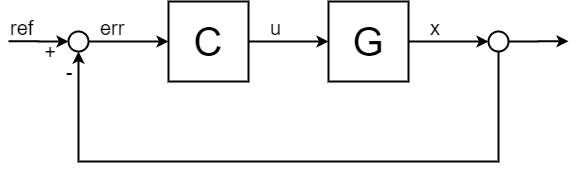
\includegraphics[width=0.6\textwidth]{4-examples/feedback.png}
            \caption{Feedback loop diagram}
            \label{fig:feedback}
        \end{figure}

        As Control System Designer only works with \ac{siso} systems, the next step is to choose which output one desires to analyse. In case of Example Model it does not make a difference which axis is chosen. This task can be performed with \verb|getSISOSystem| described in \autoref{sec:scripts}.
        
        After setting it up in Control System Designer, it shows Bode plots, Root Locus diagram and Step Response plot for the system. Using provided tools one can set up desired form of the controller, and edit Bode plots and Root Locus diagram until desired response is achieved. It was assumed that the controller needs a complex pole and a real zero, to be able to follow reference signal during tracking. Also, since the noise in gyroscopes might be causing the plant to drift too much, the desired system has to have a larger real part of the pole pole than zero. After setting it up and using Bode Editor to get high enough gain and phase margin, as seen on \autoref{fig:bode1}.

        \begin{figure}[H]
            \centering
            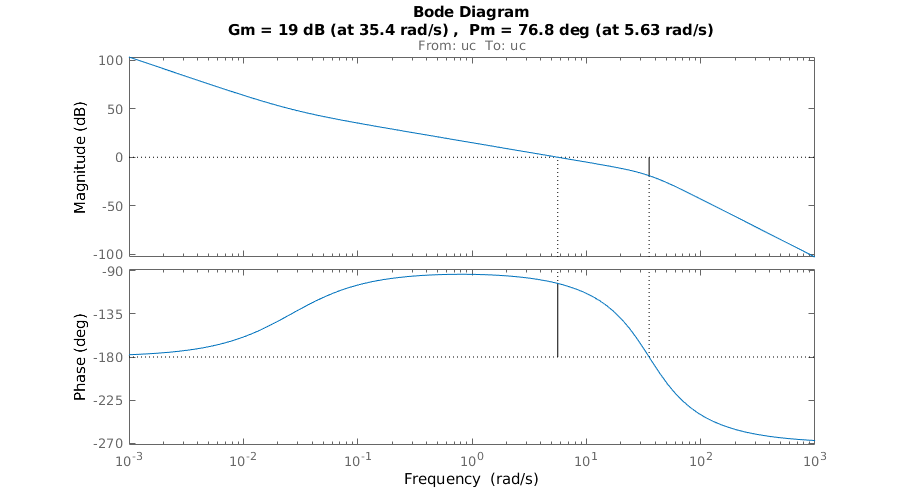
\includegraphics[width=1\textwidth]{4-examples/bode1.png}
            \caption{Bode plot of tuned system}
            \label{fig:bode1}
        \end{figure}

        The acquired controller form has following transfer function:
        
        \begin{equation}
            C(s)=10200\frac{1+10s}{1+0.33s}
        \end{equation}

        Which turned out to be a very aggressive controller, with step response presented on \autoref{fig:bode_step1}.

        \begin{figure}[H]
            \centering
            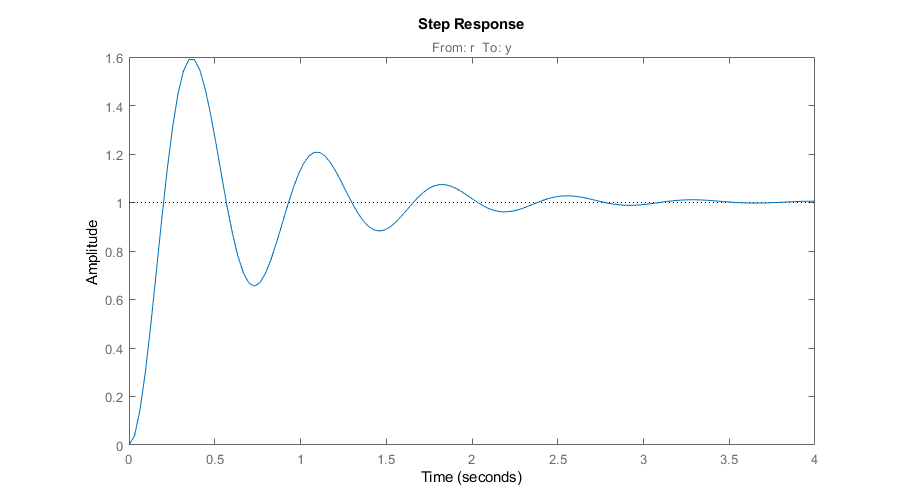
\includegraphics[width=1\textwidth]{4-examples/step1.png}
            \caption{Step response of tuned system}
            \label{fig:bode_step1}
        \end{figure}
                         
        \begin{figure}[H]
            \centering
            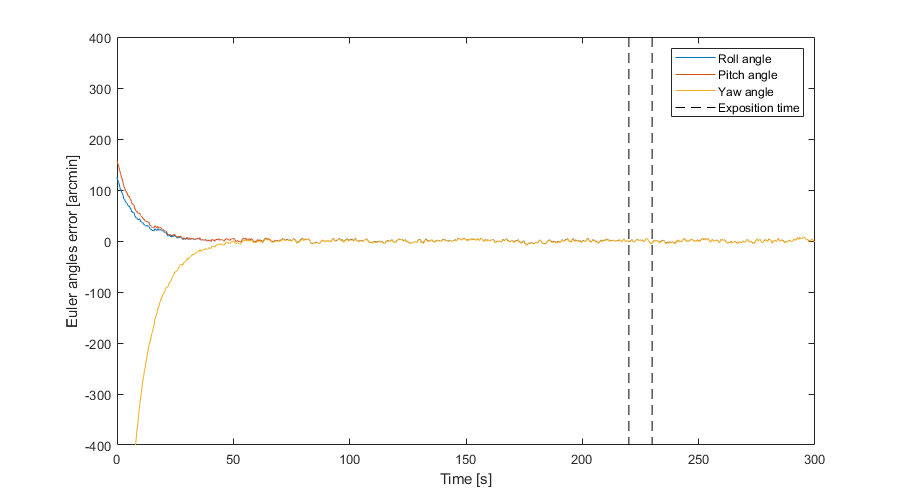
\includegraphics[width=1\textwidth, height=160px]{4-examples/bode_error.png}
            \caption{Plot of Euler angle error against reference angles, derived from geographical coordinates and satellite position}
            \label{fig:bode_error}
        \end{figure}
                     
        \begin{figure}[H]
            \centering
            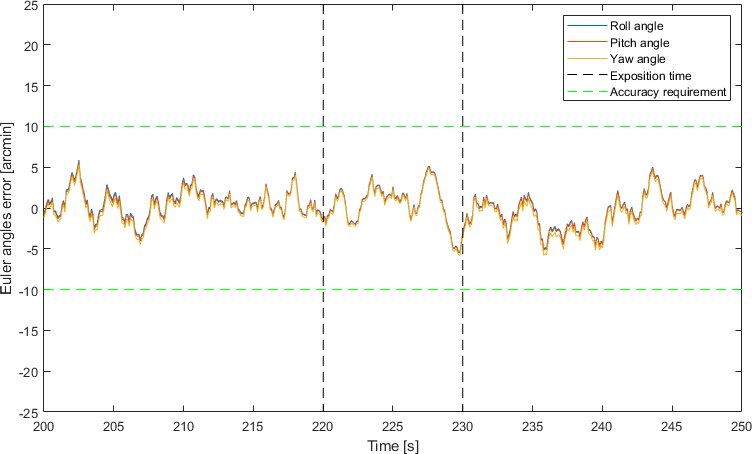
\includegraphics[width=1\textwidth, height=160px]{4-examples/bode_zoom.png}
            \caption{Plot of Euler angle error against reference angles, derived from geographical coordinates and satellite position, in focus on time between 200 and 250 seconds}
            \label{fig:bode_zoom}
        \end{figure}
        
        In the end Figures \ref{fig:bode_error} and \ref{fig:bode_zoom} present the performance of new controller, which was comparable with the one designed by empirical methods, with slight advantage on using the one tuned with Control System Designer. Figures \ref{fig:example_bode} and \ref{fig:example_step} contain, for comparison, Bode and Step Response plots generated for controller from \autoref{sec:simple_spacecraft}.

        \begin{figure}[H]
            \centering
            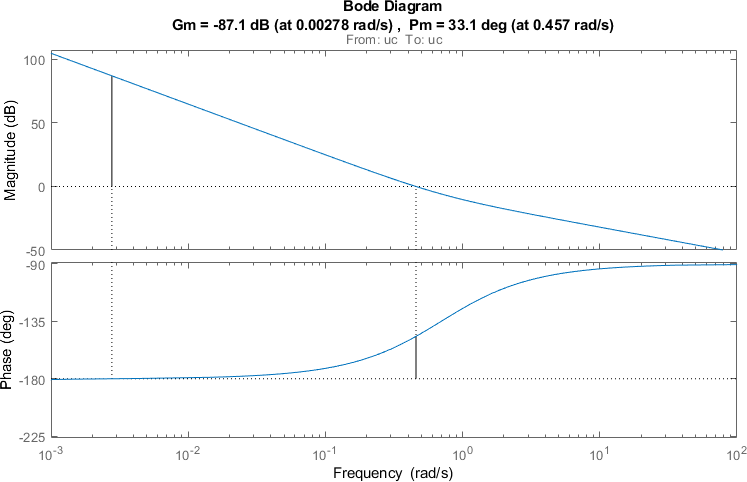
\includegraphics[width=1\textwidth]{4-examples/example_bode.png}
            \caption{Bode plot of PID controller from \autoref{sec:simple_spacecraft}}
            \label{fig:example_bode}
        \end{figure}

        \begin{figure}[H]
            \centering
            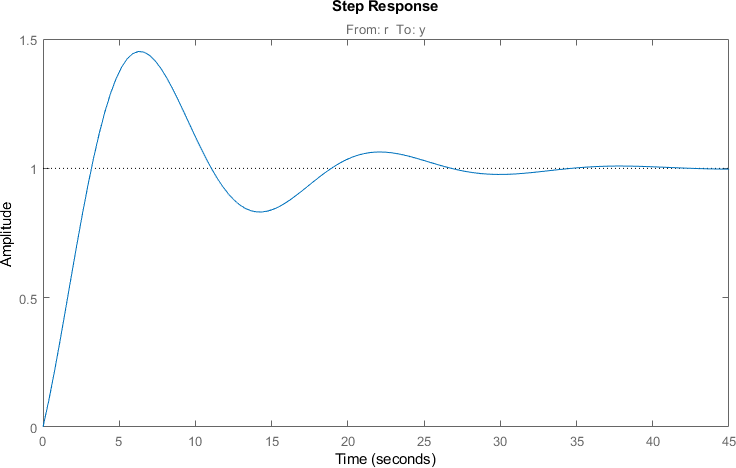
\includegraphics[width=1\textwidth]{4-examples/example_step.png}
            \caption{Step Response plot of PID controller from \autoref{sec:simple_spacecraft}}
            \label{fig:example_step}
        \end{figure}




        
    % \subsubsection{Long term simulation}
    %     \dots\textit{plots and description}\dots

    \subsubsection{Contingency scenarios simulation}
        \ac{scars} provides an easy ways of testing various contingency scenarios, which means it is possible to quickly adapt the simulation to represent redundant structures, by swapping one sensor or actuator for another, or even by just modifying existing elements. Scenario and Example Model from \autoref{sec:simple_spacecraft} can be given as a good example. In this case,  Nan-oTorque GSW-600 reaction wheels set contains four reaction wheels, one for each Cartesian axis and one on located on direction vector $\textbf{r} = [1, 1, 1]$, which makes it possible to have 3 degrees of freedom even if one actuator is not responding.

        To adapt Example Model to this scenario, one must only change one reaction wheel block from \textbf{Reaction Wheel (1-axis, X/Y/Z)} to \textbf{Reaction Wheel (1-axis, vector)} and set the \textbf{Operating Axis} parameter to $[1\; 1\; 1]$ value (the norm is calculated from the vector, so its length is not relevant in this case).

        
